\chapter{Theory}

Uniquely determining the phase difference between the $p$- and
$d$- continuum waves requires knowledge of the relative optical
phase of the two optical fields present at the interaction.  The
goal is to determine the optical phase difference, $\phi_{2
\omega} - 2\phi_{\omega}$, between the fundamental field and its
second harmonic at the interaction region.  This can be done by
using a second non-linear crystal to generate a co-linear second
harmonic beam and then looking at the magnitude of the
interference signal between the two second harmonic
beams~\cite{Chudinov}. The method makes use of the fact that,
during second harmonic generation, the harmonic field has a
definite phase relationship to that of the fundamental.  In our
experiment, both beams leave the interaction region and travel
some distance, $d$, inside the vacuum system. They then pass
through a BBO crystal where some of the visible beam is converted
into its second harmonic. At the output of the BBO crystal there
are now two second harmonic fields that will interfere
constructively or destructively depending on their relative phase.
The amplitude of the interfering beams will go as the square of
the cosine of the phase difference between them.  Therefore, by
measuring the amplitude of the interference signal, the relative
phase between the visible and uv fields at the interaction region
can be determined.

Careful consideration must be made with respect to two things when
using this method.  The first is that, as these two focused
Gaussian beams travel from their focus into the far-field, a phase
difference will develop between them.  The second is that there
will be some phase difference between the visible beam and the
second harmonic that is created from it within the BBO.  If these
are both accounted for, the optical phase difference at the
interaction region can eventually be determined correctly.


\section{Clarification of Coordinate Systems}

In performing this experiment, it is necessary to define and
adhere to a coordinate system in order to avoid confusion.  In
most cases, it is convenient to define the coordinates with
respect to the travelling optical beam.  For these cases, a
coordinate system is defined in the following way. The positive
$z$-axis points in the direction of the beam's propagation. The
positive $y$-axis is normal to or up from the optical table, and
the $x$-axis is located accordingly to create a right-handed
coordinate system.

When dealing with crystal structures, it is often more convenient
to define a coordinate system that coincides with the particular
axes of the crystal.  The type of crystal that is under study is a
uniaxial crystal, which means that light polarized along one axis
experiences a different index of refraction than does light
polarized along the other two.  This axis will be designated the
optic axis and light polarized along it will be said to be
experiencing an extraordinary refractive index. Light polarized
along either of the other two axes will be experiencing an
ordinary refractive index. In a crystal, it is customary to
designate the optic axis as the $Z$-axis, which means that the
$X$- and $Y$-axes will be used to designate the ordinary axes. For
our purposes, the $X$- and $Y$-axes will be interchangeable.

The convention used here is to designate the laboratory
coordinates in lower case ($x,y,z$) and the crystal coordinates in
upper case ($X,Y,Z$).  A diagram of these coordinates is shown in
figure(\ref{coord}).

\begin{figure}
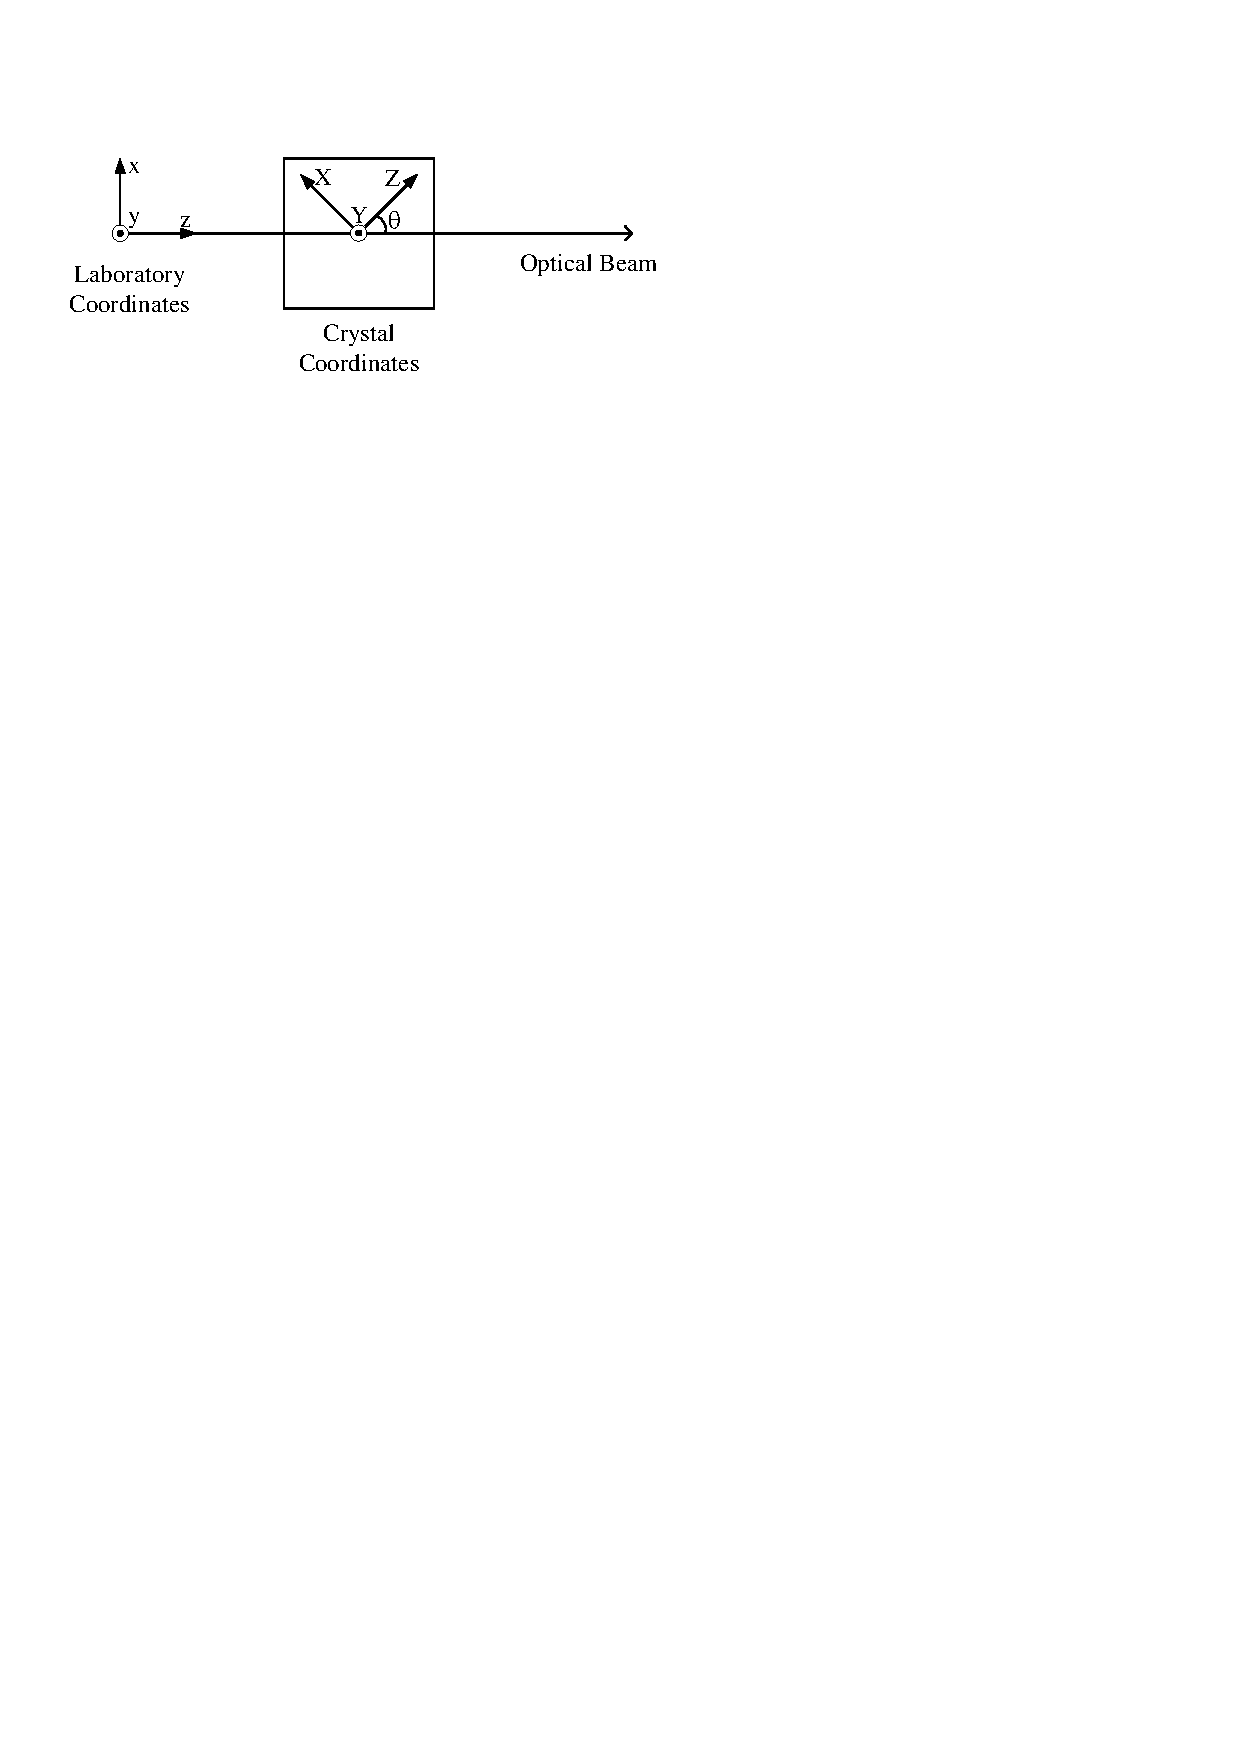
\includegraphics{coordsys2}
\caption[Definition of coordinate systems used]{Diagram showing
the two types of coordinate systems used.  Coordinates in lower
case are defined with respect to the laboratory environment and
coordinates in upper case are defined with respect to the
crystalline axes.}
\label{coord}%
\end{figure}


\section{Shift During Propagation}
\label{phaseshiftff}

We can consider the visible and uv beams to be focused Gaussian
beams.  In our reference frame, these beams are travelling in the
$+z$ direction and the beams are focused at the point $z=0$. The
focal point is placed before the interaction region at the point
$z=z_i$ for reasons discussed below.  The second BBO doubling
crystal is located some distance, $d$, after the interaction
region.  Refer to figure (\ref{opdcalc}) for an illustration of
terms used.

\begin{figure}
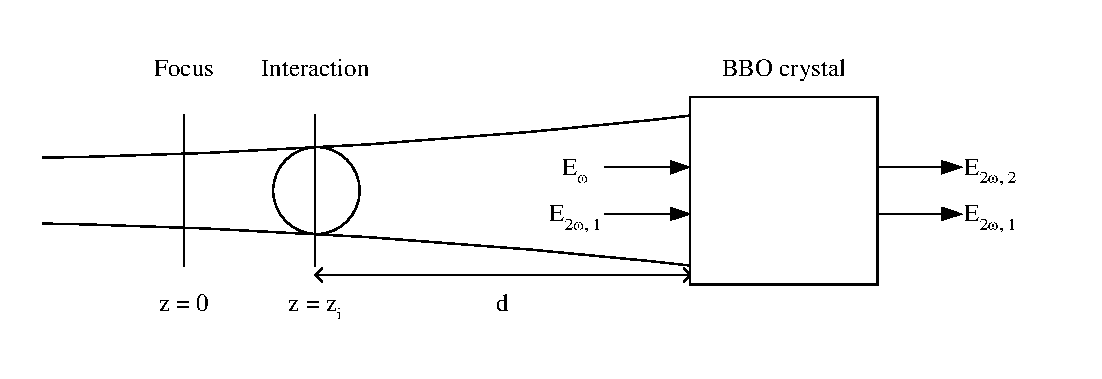
\includegraphics{focusshift}
\caption[Method for determining interaction optical phase
Difference]{Illustration of the method used to determine the
Optical Phase Difference at the interaction region}
\label{opdcalc}
\end{figure}


If we assume an electric field of the form $E(z)=E_oe^{i\phi(z)}$
then, for a Gaussian beam, the phase changes with propagation
according to~\cite{Verdeyen}

\begin{equation}\label{phiz}
\phi(z)=-kz+\arctan{\left[\frac{z}{z_o}\right]},
\end{equation} where $k$ is the wave vector of the beam, and $z_o$ is the beam's
confocal parameter. It should be noted that a second harmonic beam
will have both the same focal point and the same value of $z_o$ as
the fundamental wave from which it was created~\cite{Kleinman}.

We are ultimately interested in determining the value of the
optical phase difference at the interaction region,
$\Delta\phi_{i}=\phi_{2\omega}-2\phi_\omega$.  We can say that the
change in phase between the two fields as they travel the distance
to the BBO equals the change in phase of the visible beam minus
the change in phase of the uv beam.

\begin{equation}\label{opd1}
\Delta\phi_d-\Delta\phi_{i}=\Delta\phi_{2\omega}-2\Delta\phi_\omega
\end{equation}

In the above equation, $\Delta\phi_{2\omega}$ and
$\Delta\phi_\omega$ can be determined by using the fact that these
are focused Gaussian beams and they obey equation (\ref{phiz}).
Phase difference during propagation due to dispersion can be
ignored since the two beams are travelling in a high vacuum
environment which can be considered effectively free from
dispersion.

Knowing this, $\Delta\phi_{2\omega}$ in equation (\ref{opd1}) can
be found.

\begin{eqnarray}
\Delta\phi_{2\omega}& & = \left. \phi_{2\omega} \right|_{z=z_i+d} - \left. \phi_{2\omega} \right|_{z=z_i} \\
& & = \left[ -k_{2\omega}(z_i+d)+\arctan{\frac{z_i+d}{z_o}}
\right] - \left[ -k_{2\omega}z_i+\arctan{\frac{z_i}{z_o}} \right]
\label{opd2}
\end{eqnarray}

Similarly,

\begin{equation}\label{opd3}
\Delta\phi_\omega = \left[
-k_{\omega}(z_i+d)+\arctan{\frac{z_i+d}{z_o}} \right] - \left[
-k_{\omega}(z_i)+\arctan{\frac{z_i}{z_o}} \right].
\end{equation}

Since the uv beam has double the frequency of the visible beam,
the wave vectors of the two beams are related by:
$k_{2\omega}=2k_\omega$.  Accounting for this and substituting
equations (\ref{opd2}) and (\ref{opd3}) into equation (\ref{opd1})
yields

\begin{equation}\label{opd4}
\Delta\phi_{d}-\Delta\phi_{i}=-\arctan{\frac{z_i+d}{z_o}}+\arctan{\frac{z_i}{z_o}}.
\end{equation}

As $d$ becomes large relative to $z_o$, the the first term of
equation (\ref{opd4}) approaches $-\frac{\pi}{2}$.  In our
experimental setup, $z_o$ is on the order of a few millimeters and
$d$ is about 40 cm and so the first term will be taken as
$-\frac{\pi}{2}$.

If we look at the second term of equation (\ref{opd4}), we can see
the reason for placing the focus slightly before the interaction
region.  The arc tangent function is rapidly varying when its
argument approaches zero, therefore, choosing a value of $z_i$
that is very small could potentially introduce a large amount of
error in the final calculation of the phase difference.  If $z_i$
is chosen to be a bit larger, small errors in the location of the
focus will have less of an overall impact on the phase
measurement.  In the end, the phase difference will have to be
adjusted by this factor.


\section{Shift during Second Harmonic Generation}

In second harmonic generation (SHG), the newly generated field
will have a definite phase relationship to that of its driving
field. In general, this phase difference is non-zero and so it
must be determined in order for us to determine the phase
relationship between the visible and uv beams at the interaction.
To calculate this, we must look at the second harmonic generation
process.

In our experiment, a second harmonic field is generated using the
nonlinear crystal $\beta$-Barium Borate or BBO.  It is classified
as a negative uniaxial crystal and it has a crystal class of 3$m$.
The crystal used was cut for Type I SHG at a phase matching angle
that corresponds to the fundamental wavelength of 560nm. In Type I
SHG, the fundamental and second harmonic fields are linearly
polarized and perpendicular to each other.  The phase matching
angle, $\theta$, is the angle between the optic axis of the
crystal and the propagation direction of the optical beam at which
both the fundamental and second harmonic beams have the same phase
velocity within the crystal.  In BBO, this angle is $44.4^\circ$
for a fundamental wavelength of 560nm.

\subsection{Nonlinear Optics Background}
\label{NLO}%

The nonlinear effects arise from the fact that the material
exhibits a non-linear susceptibility.  In general, the
polarization of a material, $P$, may be described by

\begin{equation}\label{pol}
P=\epsilon_o \chi E,
\end{equation} where $\chi$ is known as the susceptibility of the material, which
may be non-linear.  Expanding equation (\ref{pol}) for the case of
a non-linear susceptibility yields

\begin{equation}\label{polexpansion}
\begin{array}{cccccccc}
P&=&P^{(1)}&+&P^{(2)}&+&P^{(3)}&+ ...\\
&=&\epsilon_o\chi^{(1)}E&+& \epsilon_o\chi^{(2)}E^2&+& \epsilon_o\chi^{(3)}E^3&+ ... \\
\end{array}
\end{equation}

We will be primarily concerned with the second order
susceptibility, $\chi^{(2)}$, since it contributes to second
harmonic generation and it offers a far greater contribution than
do all other higher order terms.  In general, $\chi^{(2)}$ is a
second order tensor.  Under certain symmetry conditions and using
the relation $d_{ijk}=\frac{1}{2}\chi^{(2)}_{ijk}$, equation
(\ref{polexpansion}) can be written in the following condensed
form which accounts for all possible orientations.~\cite{RWBoyd}


\begin{equation}\label{darray}
\left[ \begin{array}{c} P_X \\
P_Y \\
P_Z \end{array} \right]= 2 \left[ \begin{array}{cccccc}
d_{11} & d_{12} & d_{13} & d_{14} & d_{15} & d_{16} \\
d_{21} & d_{22} & d_{23} & d_{24} & d_{25} & d_{26} \\
d_{31} & d_{32} & d_{33} & d_{34} & d_{35} & d_{36} \\
\end{array}\right]
\left[ \begin{array}{c} E_X^2 \\
E_Y^2 \\
E_Z^2 \\
2 E_Y E_Z \\
2 E_X E_Z \\
2 E_X E_Y \\
\end{array} \right],
\end{equation} where $E_i$ is the magnitude of the electric field polarized in
the $i$ direction.  For a fixed polarization and propagation
direction, equation (\ref{darray}) may be further abbreviated to
the form

\begin{equation}\label{P2dE}
P^{(2)}(z,t)=2 d_{eff}E^2(z,t).
\end{equation}

If we assume an electric field of form, $\label{efield} E(z,t) =
\frac{1}{2} \left[ Ee^{i(\omega t-kz)} + c.c.\right]$, and take
the square of it, equation(\ref{P2dE}) becomes

\begin{equation}\label{pol2}
P^{(2)}=2 d_{eff} \left[ Ee^{2i(\omega t-kz)} + c.c. + 2\left| E
\right|^2 \right].
\end{equation}

This nonlinear polarization consists of two parts.  One part, $2
d_{eff} \left[ Ee^{2i(\omega t-kz)} + c.c. \right]$, consists of a
field oscillating at twice the original frequency which is
responsible for second harmonic generation.  The other part, $2
d_{eff} \left[ 2\left| E \right|^2 \right]$, contributes to what
is known as optical rectification.  It can be seen that this is a
polarization that does not vary with time.

\subsection{Second Harmonic Generation Process}
\label{SHG}

We now want to relate the electric field of the fundamental beam
entering the crystal to the second harmonic that is generated.
This can be done through use of Maxwell's equations and the wave
equation.

\begin{equation}\label{waveeqn}
-\nabla^2 E + \frac{1}{c^2} \frac{\partial^2}{\partial t^2} E =
\frac{-4\pi}{c^2} \frac{\partial^2 P}{\partial t^2}
\end{equation}


By using an electric field of the form $\label{efield}
E_{\omega}(z,t) = \frac{1}{2} \left[ Ee^{i(\omega t-kz)} + c.c.
\right]$ and equation(\ref{P2dE}),  and by making the
approximations of perfect phase matching and an undepleted
fundamental beam, equation(\ref{waveeqn}) reduces to~\cite{Yariv}

\begin{equation}\label{shgeqn}
E_{2\omega}= -i \omega \sqrt{\frac{\mu_o}{\epsilon}} d_{eff}
E_{\omega} E_{\omega} L.
\end{equation}

In the above equation, $\omega$ is the fundamental frequency,
$\mu_o$ is the magnetic susceptibility of free space, $\epsilon$
is electric permeability of the crystal, and $L$ is the length of
the crystal. The amplitudes of the second harmonic and fundamental
fields are given by $E_{2\omega}$ and $E_{\omega}$, respectively.
Also, $d_{eff}$ is defined as half of the second order nonlinear
susceptibility. According to Eimerl~\cite{Eimerl}, in crystal of
class 3$m$, $d_{eff}$ can be found by

\begin{equation}\label{deff}
d_{eff}=d_{31}\sin{\theta} - d_{22}\cos{\theta}\sin{3\phi},
\end{equation} where $\theta$ is the angle between the beam's wave vector and the
crystalline $Z$-axis and $\phi$ is the angle between the wave
vector and the crystal's $X$-$Z$ plane.  The crystal used for this
experiment is cut, for a beam with normal incidence to the
surface, with angles of $\theta=44.4^\circ$ and $\phi=0^\circ$.

From equation (\ref{shgeqn}), it can be seen that the phase of the
second harmonic field differs from that of the fundamental due to
the \(-i\) factor in equation (\ref{shgeqn}). This phase may also
be affected by the sign on \(d_{eff}\) which may be either
positive or negative, and depends on the relative orientation
between the crystal's optic axis and beam direction. Overall, this
correlates to a phase shift during SHG of either $-\frac{\pi}{2}$
or $+\frac{\pi}{2}$.  Combining this with the result of section
(\ref{phaseshiftff}) yields an overall phase shift from the beam's
focus to the phase detector of either $0$ or $\pi$.  In order to
resolve this ambiguity, we must determine the sign of $d_{eff}$.

It can be seen in equation (\ref{pol2}) that the term $d_{eff}$ is
common to both the second harmonic generation and the optical
rectification processes.  Therefore, if the sign of $d_{eff}$ can
be determined by measuring the optical rectification, then it will
also be known for the second harmonic generation process.

In summary, if we combine the results of sections
(\ref{phaseshiftff}) and (\ref{SHG}) we can arrive at an
expression for the total phase shift, $\Delta\phi_{total}$, that
occurs between the fundamental and second harmonic in travelling
from the interaction to the phase detector.

\begin{equation}
\begin{array}{cccccc}
\Delta\phi_{total}&=&-\arctan{\frac{z_i+d}{z_o}}&+&\angle \left[-i \cdot \mbox{sign}(d_{eff}) \right] &\\
                  &\approx& -\frac{\pi}{2}       &+&\angle \left[-i \cdot \mbox{sign}(d_{eff})  \right]&\mbox{for}\ z_i+d\gg z_o\\
                  &=& \left\{ \begin{array}{cccccc}
                  -\frac{\pi}{2}&+& -\frac{\pi}{2}&=&\pi &\mbox{for}\ d_{eff} >  0 \\
                  -\frac{\pi}{2}&+& \frac{\pi}{2}&=&0 &\mbox{for}\ d_{eff} < 0
                  \end{array} \right.
\end{array}
\end{equation}

\subsection{Optical Rectification}

Optical rectification is the process of generating a DC electric
field from a time-varying optical field.  An expression for the
polarization that arises from an optical rectification process was
derived in section (\ref{NLO}).

\begin{equation}\label{ORpol}
P_{DC}^{(2)}=2d_{eff} \left| E\right|^2.
\end{equation}

In our experiment, linearly polarized light is used in a Type I
phase matching configuration and this generates both a second
harmonic signal and an optical rectification signal.  The two
generated fields will have polarization perpendicular to that of
the input field. Let us assume that the input field is polarized
in the $y$-direction and that it is intersecting the crystal's
optic axis and some angle, $\theta$.  The exact orientation of the
crystal axes is not known, so an orientation is assumed for the
purposes of this derivation.  The angle that the wave vector makes
with the crystal's optic axis is known, however, due to the phase
matching condition for generation of second harmonic.  The
relative orientations of the crystalline axes and the laboratory
coordinates are shown in figure (\ref{crysorient}).

\begin{figure}
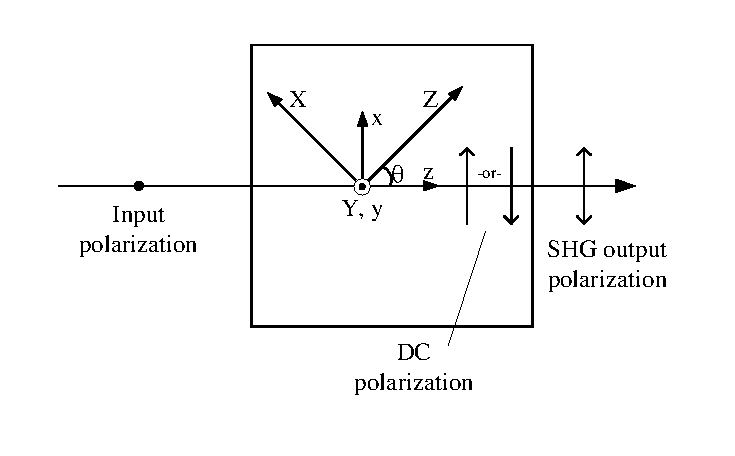
\includegraphics{polcryst}
\caption[Relative orientation of crystal and laboratory coordinate
systems]{Diagram of the relative orientations of the crystal and
laboratory coordinate systems}
\label{crysorient}%
\end{figure}

Since the beam is propagating in the $z$-direction, we can arrive
at an expression for the resulting DC polarization, written in the
laboratory coordinate system.  In order to obtain this expression,
we begin with the equation relating polarization to electric field
that was given in equation (\ref{darray}).  For a specific crystal
class, certain symmetry conditions may restrict certain values in
the $d_{ij}$ matrix to be zero or equal to other values in the
matrix. Since we are considering specifically a BBO crystal we may
use the reduced form for crystals of class 3$m$, of which BBO is a
member~\cite{RWBoyd}.

\begin{equation}\label{BBOdarray}
\left[ \begin{array}{c} P_X \\
P_Y \\
P_Z \end{array} \right]= 2 \left[ \begin{array}{cccccc}
0 & 0 & 0 & 0 & d_{15} & -d_{22} \\
-d_{22} & d_{22} & 0 & d_{15} & 0 & 0 \\
d_{31} & d_{31} & d_{33} & 0 & 0 & 0 \\
\end{array}\right]
\left[ \begin{array}{c} E_X^2 \\
E_Y^2 \\
E_Z^2 \\
2 E_Y E_Z \\
2 E_X E_Z \\
2 E_X E_Y \\
\end{array} \right].
\end{equation}

Note that the indices are given in terms of the crystal coordinate
axes.  Since the input field consists only of an electric field
linearly polarized in the $Y$-direction, equation
(\ref{BBOdarray}) reduces to

\begin{equation}
\label{crystalpol}
\begin{array}{ccc}
P_Y &=& 2d_{22}E_Y^2 \\%
P_Z &=& 2d_{31}E_Y^2. \end{array}.
\end{equation}

From this, we are interested only in the component of the
polarization that is in the $x$-direction in our laboratory
coordinate system.  In other words, we want the component that is
orthogonal to the input field and the propagation direction, which
is the result of a Type I process.  Transforming equation
(\ref{crystalpol}) into the laboratory coordinate system, the
polarization in the $x$-direction is given by

\begin{equation}
P_x=2d_{31} \sin{\theta} E_y^2,
\end{equation} and the DC polarization corresponding to this is

\begin{equation} \label{ORpolsign}
P_x=2d_{31} \sin{\theta} \left| E_y\right|^2 .
\end{equation}


This result can be verified by comparing to equation (\ref{P2dE})
and recognizing that $d_{eff}=d_{31} \sin{\theta}$ for $\phi=0$
from equation(\ref{deff}).  Since we do not know the actual
orientation of the crystal's positive $Z$-axis, we can say that we
do not know the sign of $\sin{\theta}$, and we therefore do not
know the sign of $d_{eff}$.  The problem of finding the sign of
$d_{eff}$ now comes to determining the direction of the DC
polarization that is developed in the crystal.

In order to measure this DC polarization, conducting electrodes
are placed on the sides of the crystal perpendicular to the
expected DC polarization vector.  The polarization will be
developed within the area of the laser beam in the crystal.  This
polarization corresponds to some density of dipoles, all oriented
in the same direction.  Within the crystal, this will appear as a
separation of charge with one edge of the laser beam appearing to
have a positive charge and the other appearing to have a negative
charge.  These charges will induce opposite charges on the
conducting electrodes, and thus there will be a voltage difference
between the two electrodes which can be measured.  An illustration
of this is shown in figure (\ref{polcharge}).

\begin{figure}
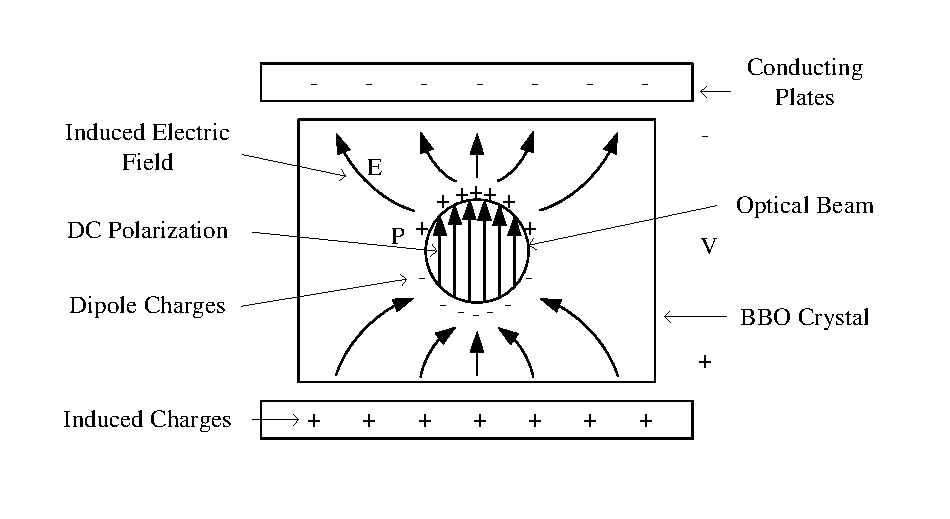
\includegraphics{polcharge}
\caption[Effect of DC polarization in BBO crystal]{Method used to
detect the polarization direction.  The DC polarization causes a
separation of charge within the crystal which, in turn, induces
charges on the conducting plates.  The difference in charge on the
plates corresponds to a voltage and the direction of the voltage
drop can be used to find the polarization direction.}
\label{polcharge}%
\end{figure}

There are two possible cases that may arise, corresponding to
possible signs of $d_{eff}$. Either the measured voltage will
correspond to a DC field which points in the positive
$x$-direction or in the negative $x$-direction. It can be seen
from equation (\ref{ORpolsign}) that a positive value of $d_{eff}$
will yield a polarization in the positive $x$-direction and a
negative value of $d_{eff}$ will yield a polarization in the
negative $x$-direction. An illustration of these two cases is
shown in figure (\ref{ORresult}).


\begin{figure}
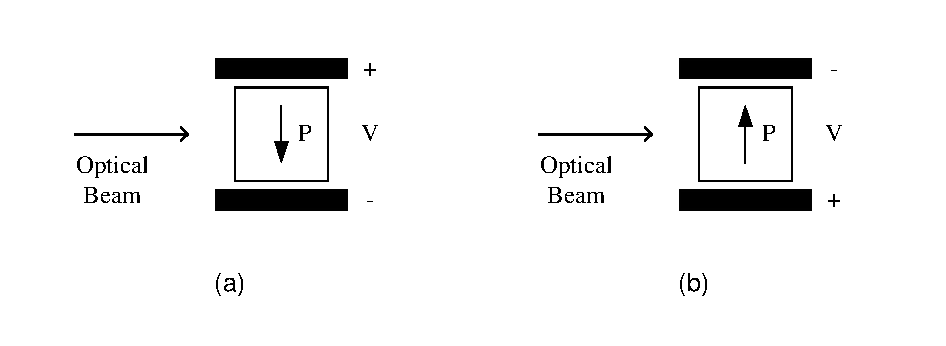
\includegraphics{ORresult}
\caption[Possible results of optical rectification
measurement]{Diagram showing the two possible results of an
optical rectification measurement, including the resulting induced
voltage.}
\label{ORresult}%
\end{figure}
